\documentclass[sigconf]{acmart}

\usepackage{graphicx}
\usepackage{caption}
\usepackage{subcaption}
\usepackage{mathtools}
\usepackage{algpseudocode}
\usepackage{algorithm}
\usepackage{algorithmicx}
\usepackage{graphicx}
\usepackage{hyperref}
\usepackage{textcomp}



%\usepackage{booktabs} % For formal tables


% Copyright
%\setcopyright{none}
%\setcopyright{acmcopyright}
%\setcopyright{acmlicensed}
%\setcopyright{rightsretained}
%\setcopyright{usgov}
%\setcopyright{usgovmixed}
%\setcopyright{cagov}
%\setcopyright{cagovmixed}


% DOI
%\acmDOI{10.475/123_4}

% ISBN
%\acmISBN{123-4567-24-567/08/06}

%Conference
\acmConference[SECR'17]{Software Engineering Conference Russia}{October 2017}{St. Petersburg, Russia} 
\acmYear{2017}
\copyrightyear{2017}

%\acmPrice{15.00}


\begin{document}

\newtheorem{mytheorem}{Theorem}

\algrenewcommand\algorithmicindent{0.5em}
\algnewcommand\algorithmicswitch{\textbf{switch}}
\algnewcommand\algorithmiccase{\textbf{case}}
\algnewcommand\algorithmicassert{\texttt{assert}}
\algnewcommand\Assert[1]{\State \algorithmicassert(#1)}
% New "environments"
\algdef{SE}[SWITCH]{Switch}{EndSwitch}[1]{\algorithmicswitch\ #1\ \algorithmicdo}{\algorithmicend\ \algorithmicswitch}
\algdef{SE}[CASE]{Case}{EndCase}[1]{\algorithmiccase\ #1}{\algorithmicend\ \algorithmiccase}

\algtext*{EndSwitch}
\algtext*{EndCase}
\algtext*{EndWhile}% Remove "end while" text
\algtext*{EndIf}% Remove "end if" text
\algtext*{EndFor}% Remove "end for" text
\algtext*{EndFunction}% Remove "end function" text

\newif\ifboldnumber
\newcommand{\boldnext}{\global\boldnumbertrue}

% Default definition is \footnotesize#1:
\algrenewcommand\alglinenumber[1]{%
  \footnotesize\ifboldnumber\bfseries\fi\global\boldnumberfalse#1:}


\title{Context-Free Path Querying with Structural Representation of Result}
%\titlenote{Produces the permission block, and
%  copyright information}
%\subtitle{Extended Abstract}
%\subtitlenote{The full version of the author's guide is available as
%  \texttt{acmart.pdf} document}


\author{Semyon Grigorev}
\affiliation{%
  \institution{Saint Petersburg State University}
  \streetaddress{7/9 Universitetskaya nab.}
  \city{St. Petersburg} 
  \state{Russia} 
  \postcode{199034}
}
\email{semen.grigorev@jetbrains.com}

\author{Anastasiya Ragozina}
\affiliation{%
  \institution{Saint Petersburg State University}
  \streetaddress{7/9 Universitetskaya nab.}
  \city{St. Petersburg} 
  \state{Russia} 
  \postcode{199034}
}
\email{ragozina.anastasiya@gmail.com}


% The default list of authors is too long for headers}
%\renewcommand{\shortauthors}{B. Trovato et al.}


\begin{abstract}
Graph data model and graph databases are popular in such areas as bioinformatics, semantic web, and social networks.
One specific problem in the area is a path querying with constraints formulated in terms of formal grammars.
The query in this approach is written as a grammar and paths querying is graph parsing with respect to the grammar.
There are several solutions to it, but they are based mostly on CYK or Earley algorithms which impose some restrictions in comparison with other parsing techniques, and employing of advanced parsing techniques for graph parsing is still an open problem.
In this paper we propose a graph parsing technique which is based on generalized top-down parsing algorithm (GLL) and allows one to build finite structural query result representation with respect to the given grammar in polynomial time and space for arbitrary context-free grammar and graph.
\end{abstract}

%
% The code below should be generated by the tool at
% http://dl.acm.org/ccs.cfm
% Please copy and paste the code instead of the example below. 
%
\begin{CCSXML}
<ccs2012>
<concept>
<concept_id>10002951.10002952.10002953.10010146</concept_id>
<concept_desc>Information systems~Graph-based database models</concept_desc>
<concept_significance>500</concept_significance>
</concept>
<concept>
<concept_id>10002951.10002952.10003197.10010825</concept_id>
<concept_desc>Information systems~Query languages for non-relational engines</concept_desc>
<concept_significance>500</concept_significance>
</concept>
<concept>
<concept_id>10003752.10003766.10003771</concept_id>
<concept_desc>Theory of computation~Grammars and context-free languages</concept_desc>
<concept_significance>300</concept_significance>
</concept>
<concept>
<concept_id>10011007.10011006.10011041.10011688</concept_id>
<concept_desc>Software and its engineering~Parsers</concept_desc>
<concept_significance>300</concept_significance>
</concept>
</ccs2012>
\end{CCSXML}

\ccsdesc[500]{Information systems~Graph-based database models}
\ccsdesc[500]{Information systems~Query languages for non-relational engines}
\ccsdesc[300]{Theory of computation~Grammars and context-free languages}
\ccsdesc[300]{Software and its engineering~Parsers}

\keywords{Graph database, path query, graph parsing, context-free grammar, top-down parsing, GLL, LL}

%\acmBadgeR{artifacts_available}

\maketitle

\section{Introduction}
Graph data model and graph data bases are very popular in such areas as bioinformatics, semantic web, and social networks.
Hence, different graph structured data analysis problems are stated and appropriate solutions for these problems are required.
%Extraction of paths which satisfy specific constraints may be useful for investigation of graph structured data and for detection of relations between data items.
One specific problem---path querying with constraints---is usually formulated in terms of formal grammars and is called formal language constrained path problem~\cite{FLCpathProblem}.

Classical parsing techniques can be used to solve formal language constrained path problem and thus the more common problem---graph parsing. 
Graph parsing may be required in graph data base querying, formal verification, string-embedded language processing, and any other areas where graph structured data is used. 

%Though constrains formulated in terms of regular languages is widely used, using of more powerful context-free grammars for graph querying is in active research: recent results is context-free extension for SPARQL~\cite{CFGonRDF} and research of Jelle Hellings~(\cite{Hellings16,ConjCFPathQuery}).

Existing solutions in context-free graph querying field usually employ such parsing algorithms as CYK or Earley~(for example~\cite{ConjCFPathQuery,CFGonRDF,GraphQueryWithEarley}). 
These algorithms are simple, but impose restrictions.
For example, CYK algorithm demands the input grammar to be transformed into Chomsky normal form causing performance issues, since parsing time depends on grammar size which significantly increases during the transformation.
Such algorithms as GLR and GLL process arbitrary context-free grammars, thus performance may be improved by employing them for graph parsing problem.
%Moreover, Earley-based graph parsing algorithm, which proposed in~\cite{GraphQueryWithEarley}, has restrictions on processing graphs with cycles: it is required to specify maximal length of path for parsing termination.
Other properties of parsing algorithms also affect performance: for example, in~\cite{Hellings16} author expects that it is possible to improve evaluation of queries for a given pair of nodes by using top-down directed parsing algorithm.
Both CYK and Earley parsing algorithms are bottom-up, CYK is undirected, and Earley-based implementation~\cite{GraphQueryWithEarley} is known to have issues with cycles processing. 
In this paper we show this assumption is true.
We also provide a positive answer to the question of applicability of advanced parsing techniques stated in~\cite{Hellings16}.
%The applicability of advanced parsing techniques~\cite{Grune} for path querying is stated as an open question in~\cite{Hellings16} and we provide positive answer to it.

Even though a set of path querying solutions has been developed~\cite{GraphQueryWithEarley,ConjCFPathQuery,QueryGraphWithData,RegularDBQuery}, query result exploration is still a challenge~\cite{hofman2015separabilityForRegQueryDebugging}, as also there is a need for simplification of complex query debugging, especially for context-free queries.
In~\cite{Hellings16}, annotated grammars are proposed as a possible solution: this representation is finite for any input data and contains information necessary for detailed result exploration.
In the paper we propose the representation more native for grammar based analysis, provided by classical parsing techniques---derivation tree---which contains exhaustive information about parsed sentence structure in terms of specified grammar.

We make the following contributions in this paper.
\begin{enumerate}
\item We propose the graph parsing algorithm based on the generalized top-down parsing algorithm---GLL~\cite{scott2010gll}---and provide its time and space complexity estimations. 
For graph $M=(V,E,L)$, space complexity is $O(|V|^3 + |E|)$ and time complexity is $O\left(|V|^3*\max\limits_{v \in V}\left(deg^+\left(v\right)\right)\right)$.
\item We answer some questions on advanced parsing techniques applicability for graph processing stated in~\cite{Hellings16}.
%Questions on possibility of advanced parsing techniques application for graph processing, and on possibility of top-down algorithms utilization for  answering queries for a given pair of nodes are stated in~\cite{Hellings16}.
%We show that all of these are possible.
%Thus we answer on first and second questions which are stated in~\cite{Hellings16}: yes, we can use advanced parsing techniques for graph parsing, and we can use top-down parsing algorithm for goal-oriented queries evaluation.
\item Proposed graph parsing algorithm constructs finite representation of parse forest containing derivation trees for all matched paths in graph. We show how this representation can be used for realistic problems solving.
\item We have implemented the proposed algorithm and our evaluation shows that advanced parsing techniques increase performance (up to 1000 times in some cases) as compared to CYK-based implementation, proposed in~\cite{CFGonRDF}.
\end{enumerate}

\section{Preliminaries}

In this work we are focused on the parsing algorithm, and not on the data representation, and we assume that whole input graph can be located in RAM memory in the optimal for our algorithm way.

We start by introduction of necessary definitions.
\begin{itemize}
  \item Context-free grammar is a quadruple $G=(N, \Sigma, P, S)$, where $N$ is a set of nonterminal symbols, $\Sigma$ is a set of terminal symbols, $S \in N$ is a start nonterminal, and $P$ is a set of productions. 
  \item $\mathcal{L}(G)$ denotes a language specified by grammar $G$, and is a set of terminal strings derived from start nonterminal of $G$: $L(G) = \{\omega | S \Rightarrow_{G}^{*} \omega\}$.
  \item Directed graph is a triple $M = (V,E,L)$, where $V$ is a set of vertices, $L \subseteq \Sigma$ is a set of labels, and a set of edges $E\subseteq V\times L\times V$. 
  We assume that there are no parallel edges with equal labels: for every $e_1=(v_1,l_1,v_2) \in E, e_2=(u_1,l_2,u_2) \in E$ if $v_1 = u_1$ and $v_2 = u_2$ then $l_1 \neq l_2$.
  \item $tag: E \rightarrow L$ is a helper function which allows to get tag of edge. $$tag(e = (v_1,l,v_2), e \in E) = l$$
  \item $\oplus: L^+ \times L^+ \rightarrow L^+$ denotes a tag concatenation operation.
%  \item Path $p$ in graph $M$ is a list of incident edges: 
%  \begin{align*}
%   p &= e_0,e_1,\dots,e_{n-1} \\
%     &= (v_0,l_0,v_1),(v_1,l_1,v_2),\dots,(v_{n-1},l_{n-1},v_n)
%  \end{align*}
%  where $v_i \in V$, $e_i \in E$, $e_i=(v_i,l_i,v_{i+1})$, $l_i \in L$, $|p| = n, n \geq 1$. 
%  \item $P$  is a set of paths $\{p: p \text{ path in } M\}$, where $M$ is a directed graph.
%  \item $\Omega: P \rightarrow L^+$ is a helper function which constructs a string produced by the given path. For every $p \in P$
  \item $\Omega$ is a helper function which constructs a string produced by the given path. For every $p \text{ path in } M$
  \begin{align*}
  & \Omega(p = e_{0},e_{1},\dots,e_{n-1}) = \\
  & tag (e_{0}) \oplus \dots \oplus tag (e_{n-1}).
  \end{align*}
\end{itemize}

Using these definitions, we state the context-free language constrained path querying as, given a query in form of grammar $G$, to construct the set of paths $$Q(M,G)=\{p|p \text{ is path in } M, \Omega(p) \in \mathcal{L}(G)\}.$$

Note that, in some cases, $Q(M,G)$ can be an infinite set, and hence it cannot be represented explicitly. 
In order to solve this problem, in this paper, we construct compact data structure representation which stores all elements of $Q(M,G)$ in finite amount of space and allows to extract any of them.

\subsection{Generalized LL Parsing Algorithm}\label{BasicGLL}

One of widely used classes of parsing algorithms is a LL(k)~\cite{Grune}---top-down algorithms which read input from left to right, build leftmost derivation, and use $k$ symbols for lookahead.
LL(k) parser may be implemented as deterministic pushdown automaton (DPDA).
On the other hand LL(k) parser may be implemented in recursive-descent manner: each rule transforms to function which can call functions for other rules in order specified by right hand side of corresponded rule.
In this case stack of DPDA are replaced with functions call stack.

Classical LL algorithm operates with a pointer to input (position $i$) and with a grammar slot---pointer to grammar in form $N \rightarrow \alpha \cdot x \beta $.
Parsing may be described as a transition of these pointers from the initial position ($i = 0$, $S \rightarrow \cdot \beta $, where $S$ is start nonterminal) to the final ($i = input.Length$, $s \rightarrow \beta \cdot$).
At every step, there are four possible cases in processing of these pointers. 

\begin{enumerate}
\item $N \rightarrow \alpha \cdot x \beta $, when $x$ is a terminal and $x = input[i]$. In this case both pointers should be moved to the right ($i \leftarrow i + 1$, $N \rightarrow \alpha  x \cdot \beta $).
\item $N \rightarrow \alpha \cdot X \beta $, when $X$ is nonterminal. In this case we push return address $N \rightarrow \alpha X \cdot \beta $ to stack and move pointer in grammar to position $X \rightarrow \cdot \gamma$.\label{itm:2}
\item $N \rightarrow \alpha \cdot $. This case means that processing of nonterminal $N$ is finished. We should pop return address from stack and use it as new slot.\label{itm:3}
\item $S \rightarrow \alpha \cdot $, where $S$ is a start nonterminal of grammar. In this case we should report success if $i = input.Length - 1$ or failure otherwise. 
\end{enumerate}

In the second case there can be several slots $X \rightarrow \cdot \gamma$ due to the fact that this algorithm is nondeterministic, so a strategy on how to choose one of them to continue parsing is needed.
In LL(k) algorithm lookahead is used to avoid nondeterminism, but this strategy is still not good enough because there are context-free languages for which deterministic choice is impossible even for infinite lookahead~\cite{LLnonLL}.
On the contrary to LL(k), generalized LL does not choose at all, handling all possible variants by using descriptors mechanism.
Descriptor is a quadruple $(L, s, j, a)$ where $L$ is a grammar slot, $s$ is a stack node, $j$ is a position in the input string, and $a$ is a node of derivation tree.
Each descriptor fully describes one parser state, thus instead of immediate processing of all variants, GLL store all possible branches and process them sequentially late.

The stack in parsing process is used to store return information for the parser---a state to return for continue after finishing current state processing.
%name of function which will be called when current function finishes computation. 
As mentioned before, generalized parsers process all possible derivation branches and parser must store it's own stack for every branch. 
It leads to an infinite stack growth being done naively.  
Tomita-style graph structured stack (GSS)~\cite{Tomita} combines stacks resolving this problem.
Each GSS node contains a pair of position in input and a grammar slot in GLL. 

In order to provide termination and correctness, we should avoid duplication of descriptors, and be able to process GSS nodes in arbitrary order. It is necessary to use the following additional sets for this.
\begin{itemize}
\item $R$---working set which contains descriptors to be processed. Algorithm terminates whenever $R$ is empty.
\item $U$---all created descriptors. Each time when we want to add a new descriptor to $R$, we try to find it in this set first.
This way we process each descriptor only once which guarantee termination of parsing.
\item $P$---popped nodes. Allows to process descriptors (and GSS nodes) in arbitrary order. 
\end{itemize}

%Instead of explicit code generation used in classical algorithm, we use table version of GLL~\cite{TableGLL} in order to simplify adaptation to graph processing.
%As a result, main control function is different from the original one because it should process LL-like table instead of switching between generated parsing functions.
%Control functions of the table based GLL are presented in Algorithm~\ref{mainTblFunctions}.
%All other functions are the same as in the original algorithm and their descriptions can be found in the original article~\cite{scott2010gll}.

%\begin{algorithm}[ht]
%\begin{algorithmic}[1]
%\caption{Control functions of table version of GLL}
%\label{mainTblFunctions}
%\Function{dispatcher}{ \ }
%  \If{$R.Count \neq 0$}  
%      \State{$(L,v,i,cN) \gets R.Get()$}
%      \State{$cR \gets dummy$}
%      \State{$dispatch \gets false$}
%  \Else
%      \State{$stop \gets true$}
%  \EndIf
%\EndFunction
%
%\Function{processing}{ \ }
%  \State{$dispatch \gets true$}
%  \Switch{$L$}
%  \Case{$(X \rightarrow \alpha \cdot x \beta)$ where $x = input[i + 1])$}
%       \If{$cN = dummyAST$} 
%          \State{$cN \gets \Call{getNodeT}{i}$} 
%       \Else 
%          \State{$cR \gets \Call{getNodeT}{i}$}
%       \EndIf
%       \State{$i \gets i + 1$}
%       \State{$L \gets (X \rightarrow \alpha x \cdot \beta)$}
%       \If{$cR \neq dummy$}
%          \State{$cN \gets \Call{getNodeP}{L, cN, cR}$} 
%       \EndIf
%       \State{$dispatch \gets false$}        
%  \EndCase
%  \Case{$(X \rightarrow \alpha \cdot x \beta)$ where $x$ is nonterminal}
%       \State{$v \gets$ \Call{create}{$(X \rightarrow \alpha x \cdot \beta), v, i, cN$}}
%       \State{$slots \gets pTable[x][input[i]]$}
%       \ForAll{$L \in slots$}
%          \State{\Call{add}{$L,v,i,dummy$}} 
%       \EndFor
%  \EndCase
%  \Case{$(X \rightarrow \alpha \cdot )$}
%       \State{\Call{pop}{v,i,cN}} 
%  \EndCase
%  \Case{$(S \rightarrow \alpha \cdot )$ when $S$ is start nonterminal}
%       \State{final result processing and error notification} 
%  \EndCase
%  \EndSwitch
%\EndFunction
%
%\Function{control}{}
%  \While{not $stop$}  
%      \If{$dispatch$}
%        \State{\Call{dispatcher}{ \ }}
%      \Else
%         \State{\Call{processing}{ \ }}
%      \EndIf
%  \EndWhile
%\EndFunction
%
%\end{algorithmic}
%\end{algorithm}

There can be more than one derivation tree of a string with relation to ambiguous grammar.
Generalized LL build all such trees and compact them in a special data structure Shared Packed Parse Forest~\cite{SPPF}, which will be described in the following section.

\subsection{Shared Packed Parse Forest}

Binarized Shared Packed Parse Forest (SPPF)~\cite{brnglr} compresses derivation trees optimally reusing common nodes and subtrees.
Version of GLL which uses this structure for parsing forest representation achieves worst-case cubic space complexity~\cite{gllParsingTree}.

Binarized SPPF can be represented as a graph in which each node has one of four types described below.
Let $i$ and $j$ be the start and the end positions of substring, and let us call a tuple $(i,j)$ an \textit{extension} of node.

\begin{itemize}
    \item \textbf{Terminal node} with label $(i, T, j)$.
    \item \textbf{Nonterminal node} with label $(i, N, j)$. 
    This node denotes that there is at least one derivation for substring $\alpha=\omega[i..j-1]$ such that $N \Rightarrow^*_G \alpha, \alpha = \omega[i..j-1] $.
    All derivation trees for the given substring and nonterminal can be extracted from SPPF by left-to-right top-down graph traversal started from respective node.     
    \item \textbf{Intermediate node}: a special kind of node used for binarization of SPPF. These nodes are labeled with $(i,t,j)$, where $t$ is a grammar slot.
    \item \textbf{Packed node} with label $(N \rightarrow \alpha \cdot \beta, k)$. 
    Subgraph with ``root'' in such node is one variant of derivation from nonterminal $N$ in case when the parent is a nonterminal node labeled with $(<\mkern-9mu | \mkern-9mu> (i, N, j))$.

\end{itemize}

Example of SPPF presented in figure~\ref{SPPF}. We remove redundant intermediate and packed nodes from the SPPF to simplify it and to decrease the size of structure.

\section{Graph Parsing Algorithm}

We propose a context-free language constrained path problem solution which allows to create finite representation of parse forest which contains trees for all satisfied paths in graph.
Finite representation of result set with structure related to specified grammar may be useful not only for results understanding and processing but also for query debugging especially for complex queries. 

Our solution is based on generalized LL (GLL)~\cite{scott2010gll, FastPracticalGLL} parsing algorithm which allows to process arbitrary (including left-recursive and ambiguous) context-free grammars with worst-case cubic time complexity and linear for LL grammars. 

\subsection{Generalized LL Parsing Algorithm}

In classical LL algorithm we have pointer in input and pointer in grammar of form $n \rightarrow \alpha \cdot x \beta $ --- grammar slot.
Parsing may be described as related movement this pointers from initial position. Thus in each step we have two pointers and some possible cases to process them. 

\begin{enumerate}
\item $n \rightarrow \alpha \cdot x \beta $ when $x$ is a terminal and $x = input[i]$ 
\item $n \rightarrow \alpha \cdot x \beta $ when $x$ is nonterminal
\item $n \rightarrow \alpha \cdot $
\item $s \rightarrow \alpha \cdot $
\end{enumerate}

In case (2) we can use $FIRST$ set to choose single variant. 
But sometimes it is not possible to select only one path to continue parsing and it does not allow to use LL parsing algorithm.
Generalized LL algorithm handle all possible paths in this case. 
Instead of immediate processing of all variants GLL uses descriptors mechanism to store all possible branches and process them sequentially. 
Descriptor is a quadriple $(L, s, j, a)$ where $L$ is a grammar slot, $s$ is a stack node, $j$ is a position in the input, and $a$ is a node of derivation tree. 

Stack in parsing process is used to store return information for the parser --- a name of function which would be called when current function will finish computing. 
As previously mentioned, generalized parsers process all possible derivation branches and for every branch parser must store it's own stack. It leads to infinite stack grow.  
Tomita-style graph structured stack (GSS)~\cite{Tomita} allows to combine stacks to solve this problem.
In GLL each GSS node contains a pair of position in input and grammar slot. 

Detailed description of GLL parsing algorithm is available in this article~\cite{GLL}. Pseudocode of stack and tree manipulation functions can be found in Appendix~\ref{GLLCode}.

$R$ ---   
We use table version~\cite{TableGLL} instead of code generation.

\begin{algorithm}[h]
\begin{algorithmic}[1]
\caption{Control functions}
\label{mainFunctions}
\Function{dispatcher}{}
  \If{$R.Count \neq 0$}  
      \State{$(L,v,i,cN) \gets R.Get()$}
      \State{$cR \gets dummy$}
      \State{$dispatch \gets false$}
  \Else
      \State{$stop \gets true$}
  \EndIf
\EndFunction

\Function{processing}{}
  \State{$dispatch \gets true$}
  \Switch{$L$}
  \Case{$(X \rightarrow \alpha \cdot x \beta)$ where $x = input[i + 1])$}
       \If{$cN = dummyAST$} 
          \State{$cN \gets \Call{getNodeT}{i}$} 
       \Else 
          \State{$cR \gets \Call{getNodeT}{i}$}
       \EndIf
       \State{$i \gets i + 1$}
       \State{$L \gets (X \rightarrow \alpha x \cdot \beta)$}
       \If{$cR \neq dummy$}
          \State{$cN \gets \Call{getNodeP}{L, cN, cR}$} 
       \EndIf
       \State{$dispatch \gets false$}        
  \EndCase
  \Case{$(X \rightarrow \alpha \cdot x \beta)$ where $x$ is nonterminal}
       \State{$v \gets$ \Call{create}{$(X \rightarrow \alpha x \cdot \beta), v, i, cN$}}
       \State{$slots \gets pTable[x][input[i]]$}
       \ForAll{$L \in slots$}
          \State{\Call{add}{L,v,i,dummy}} 
       \EndFor
  \EndCase
  \Case{$(X \rightarrow \alpha \cdot )$}
       \State{\Call{pop}{v,i,cN}} 
  \EndCase
  \Case{$(S \rightarrow \alpha \cdot )$ when $S$ is start nonterminal}
       \State{final result processing and error notification} 
  \EndCase
  \EndSwitch
\EndFunction

\Function{control}{}
  \While{not $stop$}  
      \If{$dispatch$}
        \State{\Call{dispatcher}{}}
      \Else
         \State{\Call{processing}{}}
      \EndIf
  \EndWhile
\EndFunction

\end{algorithmic}
\end{algorithm}

There are more than one tree for ambiguous grammar and generalized algorithms builds all derivation trees. Special data structure --- SPPF --- is used to reduce space required for tree storage.


\subsection{Shared packed parse forest}

Shared Packed Parse Forest (SPPF)~\cite{SPPF} is a special data structure for derivation forest compact representation which allow to reuse common nodes and subtrees.
As a result multiple derivation trees, which can be produced in case of ambiguous grammar, can be compressed in one SPPF with optimal reusing of common parts.  
Binarized form of SPPF proposed in~\cite{brnglr} and it allow to achieve worst-case cubic space complexity.
GLL can use SPPF~\cite{gllParsingTree} for results representation achieve cubic space complexity with binarised version.

Let we present an example of SPPF for ambiguous grammar $G_0$ (pic~\ref{grammarG0}).

\begin{figure}[h]
   \begin{center}
\begin{verbatim}
   0: s = eps
   1: s = A s B
   2: s = s s
\end{verbatim}
   \caption{Grammar $G_0$}
   \label{grammarG0}        
   \end{center}
\end{figure}


Let we parse the sentence \verb|"ABABAB"|. 
There are two different leftmost derivations of this sentence in grammar $G_0$, hence SPPF should contains two different trees and it is presented in figure~\ref{sppfSample}: result SPPF(fig. ~\ref{sppf}) and trees for derivation 1(fig.~\ref{tree1}) and derivation 2(fig.~\ref{tree2}) respectively. 
 
\begin{figure*}[ht]
    \begin{center}
    \centering
    \begin{subfigure}[b]{0.3\textwidth}
        \includegraphics[width=\textwidth]{dot/Brackets.pdf}
        \caption{SPPF}
        \label{sppf}        
    \end{subfigure}
    ~
    \begin{subfigure}[b]{0.3\textwidth}
        \includegraphics[width=\textwidth]{dot/Brackets.pdf}
        \caption{Tree for derivation 1}
        \label{tree1}        
    \end{subfigure}
    ~
    \begin{subfigure}[b]{0.3\textwidth}
        \includegraphics[width=\textwidth]{dot/Brackets.pdf}
        \caption{Tree for derivation 2}
        \label{tree2}        
    \end{subfigure}
    \caption{SPPF for sentence \textbf{\texttt{"(1)(2)(3)"}} and grammar $G_0$}
    \label{sppfSample}
    \end{center}                
\end{figure*}

Binarised SPPF can be represented as a graph where each node has one of four types which described below with corresponded graphical notation.

\begin{itemize}
    \item Node with rectangle shape labeled with $(i, T, j)$ is terminal node.     
    \item Node with oval shape labeled with $(i, N, j)$ is nonterminal node. 
    This node denote that there is at least one derivation for substring $\alpha$ from position $i$ to position $j$ in input string $\omega$ such that $N \Rightarrow^*_G \alpha, \alpha = \omega[i..j-1] $.
    All derivation trees for given substring and nonterminal can be extracted from SPPF by left-to-right top-down graph traversal started from respective node. 
    We use filled nonterminal node labeled with $(<\mkern-11mu | \mkern-11mu> (i, N, j))$ for denote that there are more then one derivations from nonterminal $N$ for substring from $i$ to $j$.
    \item Intermediate node with label $(i,t,j)$ where $t$ is a grammar slot. We use dot shape for these nodes and omit label because it is important only for SPPF constriction.
	Subgraph with root in such node is one variant of derivation in case when parent is nonterminal node with label $(<\mkern-9mu | \mkern-9mu> (i, N, j))$.
    \item Node with rectangle shape and label $(N : \gamma \cdot, k)$ is a packed node.
\end{itemize}
One of nonterminal nodes can be marked as 'root' --- node for start nonterminal. Tuple of positions $(i,j)$ which represent start and end of substring is \textit{extension} of node.

Further in our examples we will remove redundant intermediate and packed nodes from SPPF to simplify it and decrease size of structure.

\subsection{GLL-based graph parsing}

In this section we present such modification of GLL algorithm, that for input graph $M$, set of start vertices $V_s\subseteq V$, set of final vertices $V_f\subseteq V$, grammar $G_1$, it return SPPF which contains all derivation trees for all paths $p$ in $M$, such that $\Omega(p) \in L(G_1)$, and $p.start \in V_s, p.end \in V_f$.

First of all note that input string for classical parser is a linear graph, and positions in input is vertices of this graph.
This observation can be generalized to arbitrary graph with remark that in the position we have not only one next symbol, but set of labels of all outgoing edges for given vertex. 
Thus in order to use GLL for graph parsing we need to use graph vertices as position in input and modify \textbf{Processing} function to allow to process more then one "next symbol".
Required modifications presented in listing~\ref{modifAlgo}.
Small modification also required for initialization of $R$ set: it is necessary to add not only one initial descriptor but set of descriptors for all vertices in $V_s$.
All other functions can be reused from original algorithm without any changes.

\begin{algorithm}[h]
\begin{algorithmic}[1]
\caption{\textbf{Processing} function modified in order to process arbitrary directed graph}
\label{modifAlgo}
\Function{processing}{}
  \State{$dispatch \gets true$}
  \Switch{$L$}
  \Case{$(X \rightarrow \alpha \cdot x \beta)$ where $x$ is terminal}
	   \ForAll{$\{ e | e \in input.outEdges(i), tag(e) = x \}$}
	   \State{$new\_cN \gets cN$}
       \If{$new\_cN = dummyAST$} 
          \State{$new\_cN \gets \Call{getNodeT}{e}$} 
       \Else 
          \State{$new\_cR \gets \Call{getNodeT}{e}$}
       \EndIf
       \State{$L \gets (X \rightarrow \alpha x \cdot \beta)$}
       \If{$new\_cR \neq dummy$}
          \State{$new\_cN \gets \Call{getNodeP}{L, new\_cN, new\_cR}$} 
       \EndIf
	   \State{\Call{add}{L,v,target(e),new\_cN}}
	   \EndFor
  \EndCase
  \Case{$(X \rightarrow \alpha \cdot x \beta)$ where $x$ is nonterminal}
       \State{$v \gets$ \Call{create}{$(X \rightarrow \alpha x \cdot \beta), v, i, cN$}}
       \State{$slots \gets \bigcup_{e \in input.OutEdges(i)} pTable[x][e.Token]$}
       \ForAll{$L \in slots$}
          \State{\Call{add}{L,v,i,dummy}} 
       \EndFor
  \EndCase
  \Case{$(X \rightarrow \alpha \cdot )$}
       \State{\Call{pop}{v,i,cN}} 
  \EndCase
  \Case{$\_$}
       \State{final result processing and error notification} 
  \EndCase
  \EndSwitch
\EndFunction

\end{algorithmic}
\end{algorithm}

As far as we can specify sets of start and final vertices, our solution can find all paths in graph, all paths from specified vertex, all paths between specified vertices. 
Also SPPF represents a structure of paths in terms of derivation which allow to get more useful information about result. 

A bit more on correctness.!!!!! Total number of descriptors is finite. Twice in R. So, termination. Tree construction is not changed. 
\subsection{Complexity}

Time complexity estimation in terms of input graph and grammar size is quite similar to the estimation of GLL complexity provided in~\cite{gllParsingTree}.

\begin{lemma}\label{lem:Descriptors}
For any descriptor $(L,u,i,w)$ either $w = \$$ or $w$ has extension $(j,i)$ where u has index $j$.
\end{lemma}
\begin{proof}
Proof of this lemma is the same as provided for original GLL in~\cite{gllParsingTree} because main function used for descriptors creation has not been changed.
\end{proof}


\begin{mytheorem}\label{thm:GSSSpace}
The GSS generated by GLL-based graph parsing algorithm for grammar $G$ and input graph $M=(V,E,L)$ has at most $O(|V|)$ vertices and $O(|V|^2)$ edges.
\end{mytheorem}

\begin{proof}

Proof is the same as the proof of \textbf{Theorem 2} from~\cite{gllParsingTree} because structure of GSS has not been changed. 

\end{proof}

\begin{mytheorem}\label{thm:SPPFSpace}
The SPPF generated by GLL-based graph parsing algorithm on input graph $M=(V, E, L)$ has at most $O(|V|^3 + |E|)$ vertices and edges.
\end{mytheorem}

\begin{proof}
Let us estimate the number of nodes of each type.
\begin{itemize}
\item \textbf{Terminal nodes} are labeled with $(v_0, T, v_1)$, and such label can only be created if there is such $e \in E$ that $e=(v_0, T,v_1)$. 
Note, that there are no duplicate edges. 
Hence there are at most $|E|$ terminal nodes.
\item \textbf{$\varepsilon$-nodes} are labeled with $(v, \varepsilon, v)$, hence there are at most $|V|$ of them. 
\item \textbf{Nonterminal nodes} have labels of form $(v_0, N, v_1)$, so there are at most $O(|V|^2)$ of them.
\item \textbf{Intermediate nodes} have labels of form $(v_0, t, v_1)$, where $t$ is a grammar slot, so there are at most $O(|V|^2)$ of them.
\item \textbf{Packed nodes} are children either of intermediate or nonterminal nodes and have label of form $(N \rightarrow \alpha \cdot \beta, v)$.
There are at most $O(|V|^2)$ parents for packed nodes and each of them can have at most $O(|V|)$ children.
\end{itemize}

As a result, there are at most $O(|V|^3 + |E|)$ nodes in SPPF.

The packed nodes have at most two children so there are at most $O(|V|^3 + |E|)$ edges which source is packed node. 
Nonterminal and intermediate nodes have at most $O(|V|)$ children and all of them are packed nodes.
Thus there are at most $O(|V|^3)$ edges with source in nonterminal or intermediate nodes. As a result there are at most $O(|V|^3 + |E|)$ edges in SPPF.


\end{proof}

\begin{mytheorem}
The worst-case space complexity of GLL-based graph parsing algorithm for graph $M=(V,E,L)$ is $O(|V|^3 + |E|)$.
\end{mytheorem}

%\begin{proof}

Immediately follows from theorems~\ref{thm:GSSSpace} and~\ref{thm:SPPFSpace}. 

%\end{proof}


\begin{mytheorem}\label{thm:complexity}
The worst-case runtime complexity of GLL-based graph parsing algorithm for graph $M=(V,E,L)$ is $$O\left(|V|^3*\max\limits_{v \in V}\left(deg^+\left(v\right)\right)\right).$$
\end{mytheorem}

\begin{proof}

From Lemma~\ref{lem:Descriptors}, there are at most $O(|V|^2)$ descriptors. 
Complexity of all functions which were used in algorithm is the same as in proof of \textbf{Theorem 4} from~\cite{gllParsingTree} except \textbf{Processing} function in which not a single next input token, but the whole set of outgoing edges, should be processed.
Thus, for each descriptor at most $$\max\limits_{v \in V}\left(deg^+\left(v\right)\right)$$ edges  are processed, where $deg^+(v)$ is outdegree of vertex $v$.

Thus, worst-case complexity of proposed algorithm is $$O\left(V^3*\max\limits_{v \in V}\left(deg^+\left(v\right)\right)\right).$$
\end{proof}

%Also we can get averege-case complexity by calculate averege outdegree:
%\begin{align} \label{eq:avg}
%  & O\left(|V|^3*\frac {\sum\limits_{v \in V} deg^+(v)}{|V|}\right) = \nonumber \\
%  & O\left(|V|^2*\sum\limits_{v \in V} deg^+(v)\right) = \nonumber \\
%  & O\left(|V|^2*|E|\right) 
%\end{align}

We can get estimations for linear input from theorem~\ref{thm:complexity}. $\text{For any } v \in V$, $deg^+(v) \leq 1$, thus $\max\limits_{v \in V}(deg^+(v))  = 1 $ and worst-case time complexity $O(|V|^3)$, as expected. 
For LL grammars and linear input complexity should be $O(|V|)$ for the same reason as for original GLL.
 
As discussed in~\cite{modellingGLL}, special data structures, which are required for the basic algorithm, can be not rational for practical implementation, and it is necessary to find balance between performance, software complexity, and hardware resources.
As a result, we can get slightly worse performance than theoretical estimation in practice.

Note that result SPPF contains only paths matched specified query, so result SPPF size is $O(|V'|^3 + |E'|)$ where $M'=(V',E',L')$ is a subgraph of input graph $M$ which contains only matched paths.
Also note that each specific path can be explored by linear SPPF traversal. 

\section{Motivating Example}\label{motivExample}

Suppose that you are student in a School of Magic.
It is your first day in the School, so navigation in the building is a problem for you.
Fortunately, you have a map of the building (fig.~\ref{input}) and an additional knowledge about building construction:
\begin{itemize}
  \item there are towers in the school (nodes of the graph in your map);
  \item all floors of some towers connected by directed galleries (edges in your map);
  \item each gallery has a ``magic'' property: start floor is aways one more (edge label is 'b') or one less (edge label is 'b') then end floor. 
\end{itemize}

\begin{figure}[h]
    \begin{center}
        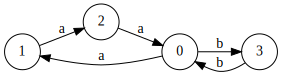
\includegraphics[width=6cm]{dot/input.pdf}
        \caption{The map of School (input graph $M$)}
        \label{input}        
    \end{center}
\end{figure}


You want to find a path from your current position to the same floor in another tower. 
Map with all such paths can help you.
But orienteering is not your forte, so it would be great if the structure of the paths were as simple as possible and all paths will have checkpoints to control your rout.

It is evident that the simplest structure of required paths is $\{ab, aabb, aaabbb, \dots\}$.
In terms of our definitions you have a graph $M=(\{0;1;2;3\},E,\{a;b\})$ (figure~\ref{input}), and you want to find all paths $p$, such that $\Omega(p) \in \{ab; aabb; aaabbb; \dots\}$ or $\Omega(p) \in a^n b^n$ where $n \geq 1$.


Unfortunately, language $\mathcal{L} = \{a^n b^n; n \geq 1\}$ is not regular which restricts the set of tools you can use. 
Another problem is the infinite size of solution, but you want to get a finite map.  
Moreover, you want to know a structure of paths with checkpoints added.

We are not aware of any existing tools which can help to solve this problem and we create a new one.
Let us to show how to get the map which help to orient in this strange School.

Fortunately, the language $\mathcal{L} = \{a^n b^n; n \geq 1\}$ is a context-free language and can be specified with context-free grammar. 
The fact that one language can be described with more than one grammar allows to add checkpoints: additional nonterminals can mark required parts of a sentence.
In our case, a desired checkpoint can be in the middle of the path.
As a result, required language can be specified by the grammar $G_1$ presented in figure~\ref{grammarG}, where $N = \{s; \text{\textit{Middle}}\}$, $\Sigma = \{a; b\}$, and $S$ is a start nonterminal.

\begin{figure}[h]
   \begin{center}
   \[
\begin{array}{rl}
   0:& S \rightarrow a \ S \ b \\
   1:& S \rightarrow Middle \\
   2:& Middle \rightarrow a \ b
\end{array}
\]

   \caption{Grammar $G_1$ for language $L=\{a^n b^n; n \geq 1\}$ with additional marker for a middle of a path}
   \label{grammarG}        
   \end{center}
\end{figure}

In the next section we present a map construction algorithm,  which solves such problems.

\section{Evaluation}

The goal of this evaluation is to assess the performance scaling of Spla on Vortex.
Due to limitations in atomic operation support within the RTL implementation, all experiments were performed using the SimX functional simulator.

\subsection{Environment}

Initial testing revealed issues with floating-point operations, which produced incorrect results for some hardware configurations.
Consequently, we limited subsequent experiments to Breadth-First Search (BFS) and Triangle Counting (TC), excluding Single-Source Shortest Path (SSSP) and PageRank.
To keep simulation times manageable, we used a single graph from the SuiteSparse matrix collection\footnote{A diverse collection of sparse matrices from various domains: \url{http://sparse.tamu.edu/}}: soc-Epinions1, with 75~888 vertices and 508~837 edges.


We conducted two series of experiments.
The first varies the number of warps and threads per warp while keeping the number of clusters and cores fixed (at 2 and 4, respectively), with the goal of selecting the best core configuration while preserving multi-core execution to account for cache effects.
The second series, using the best configuration identified in the first step, varies the number of clusters and cores per cluster to assess scaling at the core and cluster levels.
Cache sizes were set to their default values: 16 KB for $L_1$, 1 MB for $L_2$, and 2 MB for $L_3$.

We use the number of cycles reported by SimX as a performance metric.
For multi-core configurations, we report the maximum cycle count across all cores.
During the experiments, we encountered unexpected behavior in SimX that led to out-of-memory exceptions. 
Therefore, some data points are missing from the graphs below.

\subsection{Results}

In figures~\ref{fig:tc_threads_warps} and~\ref{fig:bfs_threads_warps}

\begin{figure}
    \begin{center}
        \includegraphics[width=0.49\textwidth]{pictures/TC_threads_warps.pdf}
    \end{center}
    \caption{Scaling analysis of triangle counting for varying numbers of warps and threads per warp}
    \label{fig:tc_threads_warps}
\end{figure}

\begin{figure}
    \begin{center}
        \includegraphics[width=0.49\textwidth]{pictures/BFS_threads_warps.pdf}
    \end{center}
    \caption{Scaling analysis of BFS for varying numbers of warps and threads per warp}
    \label{fig:bfs_threads_warps}
\end{figure}

Best configuration for BFS is 2 warps, 8 threads per warp (16 threads total). 
Best configuration for TC is 4 warps, 16 threads per warp (64 threads total).


\begin{figure}
    \begin{center}
        \includegraphics[width=0.49\textwidth]{pictures/BFS_cores_clusters.pdf}
    \end{center}
    \caption{Scaling analysis of BFS for varying numbers of clusters and cores per cluster}
    \label{fig:bfs_cores_clusters}
\end{figure}


Edges per core on cycle. Compare with Spla on other GPUs.

\subsection{Scaling limitations analysis}

%sum(scoreboard stalls * lsu_percent) / sum(instr) * 100
To analyze the reasons for limited scaling as the number of threads increases, we measured the average utilization of the ALU and LSU, in terms of stall cycles, for the best BFS configuration.
The results are presented in Fig.~\ref{fig:bfs_alu_stalls} and Fig.~\ref{fig:bfs_lsu_stalls}, respectively.
The data indicate that the LSU is the performance bottleneck within the core.

The same bottleneck was observed in the scaling analysis across clusters and cores.
Whether increasing cache sizes can alleviate this problem remains a question for future research.
We anticipate that careful cache size tuning may help identify a more efficient configuration.

\begin{figure}
    \begin{center}
        \includegraphics[width=0.49\textwidth]{pictures/BFS_alu.pdf}
    \end{center}
    \caption{ALU stalls on BFS for the best configuration}
    \label{fig:bfs_alu_stalls}
\end{figure}

\begin{figure}
    \begin{center}
        \includegraphics[width=0.49\textwidth]{pictures/BFS_lsu.pdf}
    \end{center}
    \caption{LSU stalls on BFS for the best configuration}
    \label{fig:bfs_lsu_stalls}
\end{figure}
\section{Conclusion and Future Work}

Platform presented.

Education. Metaprogramming, translators development, GPGPU programming, etc.

Graph parsing.

Geterogenious porgramming generalization. Hopac is better then MBP~\footnote{\url{https://vasily-kirichenko.github.io/fsharpblog/actors}}.

Research: Automatic memory management.

Data to code translation (automata can be translated into code instead of data structures in memory)

Other technical improvements: IDE support, type provider improvements, new OpenCL standard support, runtime extension, etc.
\section*{Acknowledgments}

We are grateful to the Jelle Hellings and Ekaterina Verbitskaia for their careful reading, pointing out some mistakes, and invaluable suggestions.
This work is supported by grant from JetBrains Research



\bibliographystyle{ACM-Reference-Format}
\bibliography{ContextFreeConstrainedPathFindingInGraph} 

\end{document}
